% ************ Chapter 4 ************
%\renewcommand{\chaptername}{Chapter}

\chapter{Desenho}
\label{cap:4}
\emph{Este capítulo incide na apresentação da forma como a framework Solid está até ao momento estruturada e como será estruturada a nova arquitetura proposta}

\section{Arquitetura Actual}

O Solid é um projeto open-source, envolvido numa comunidade criada e ativamente impulsionada por Tim Burners Lee. Esta comunidade dedica os seus esforços principalmente no desenvolvimento do POD como um todo, bem como documentação e ferramentas que permitem uma mais fácil integração da solução de novas aplicações. Tendo assim, como objetivo principal desenvolver e promover todo um ecosistema à volta do Solid.

\subsection{Autenticação}
A identidade dos utilizadores no Solid baseia-se em URIs WebID, estes funcionam como nomes universais que permitem identificar determinado utilizador de forma descentralizada. Segue-se um exemplo de um possível WebID:

\emph{https://john.domain.com/profile/card\#me}

Neste sentido, o Solid, tratando-se de uma plataforma descentralizada, tem requisitos diferentes da maioria das aplicações existentes. Mais propriamente, precisa de estar assente em mecanismos de autenticação \emph{cross-domain} suficientemente descentralizados e isolados de qualquer serviço ou entidade.\cite{solid_spec}

Até ao momento, o mecanismo de autenticação a ser utilizado em determinada instância de um POD, pode ser um de dois: WebID-TLS ou WebID-OIDC. Esta capacidade de abstração ao mecanismo de autenticação, permite que possam continuamente ser estudados e adotados novos mecanismos que se entenda relevantes.\cite{solid_spec}
\subsubsection{WebID-TLS}
WebID-TLS foi o primeiro mecanismo de autenticação a ser implementado no Solid. Como forma de autenticar os WebIDs, em vez das tradicionais passwords recorre a certificados criptográficos (guardados e geridos no navegador web do utilizador) para comprovar a identidade do utilizador.\cite{solid_webid-tls:}

Este mecanismo, apesar de poder ainda ser utilizado, deixou de ser a configuração por defeito para instanciações de novos PODs. Isto, porque muitos navegadores web removeram suporte ao elemento \emph{KEYGEN}, que servia como base para este protocolo gerar certificados através do navegador web.\cite{solid_webid-tls:}

\subsubsection{WebID-OIDC}
Como qualquer outro mecanismo de autenticação baseado webID, o produto final do mecanismo de autenticação. Este é baseado no protocolo OpenID connect (OIDC), adicionando passo extra que permite obter um URI WebID através de um token OIDC.\cite{solid_webid_oidc}

Seguem-se alguns dos conceitos mais relevantes neste protocolo:
\begin{itemize}
    \item \emph{User} - Utilizador humano (pode ser também uma aplicação ou serviço se estes tiverem o seu próprio webID). Também chamado \emph{Resource Owner}
    \item \emph{User-Agent} - Nome formal para navegador Web.
    \item \emph{Identity Provider (OP)} - Um servidor de identidade baseado no protocolo OpenID Connect. Pode ser utilizado o próprio POD uma instância externa.
    \item \emph{Resource Server} - Um servidor responsável por alojar recursos que o utilizador precisa eventualmente de aceder, tais como HTML, imagens, \emph{Linked Data} / \emph{RDF sources}, entre outros tipos de recursos.
    \item \emph{Relying Party (RP)} - É um POD ou uma aplicação cliente que assenta a sua lógica num token providenciado por um servidor de identidade.
    \item \emph{POD} - Unidade online de armazenamento pessoal. Este componente do sistema desempenha vários papeis na arquitetura atual: armazena informação do utilizador (actua como \emph{Resource Server}), instancia um servidor de identidade webID-OIDC e pode também actuar como \emph{Relying Party} quando um utilizador requisita recursos a partir de um token.
\end{itemize}

\begin{figure}[h]
    \begin{center}
    % Requires \usepackage{graphicx}
    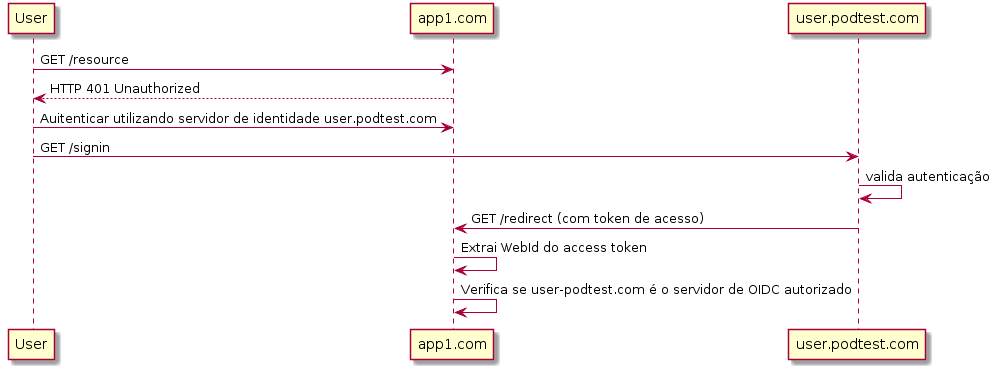
\includegraphics[width=1 \textwidth]{figures/WedId-OIDC.png}
    \caption{Diagrama de Sequência WebId-OIDC}
    \end{center}
\end{figure}

\pagebreak

Conforme é possível perceber pela figura acima, assemelha-se bastante ao protocolo OpenId Connect, adicionando dois passos extra:\cite{solid_webid_oidc}
\begin{itemize}
    \item Obter o WebId através do token de acesso
    \item Verificar se o servidor indicado para autenticação é de facto o servidor de identidade autorizado para o WebId em questão
\end{itemize}

\subsection{Autorização}

A autorização no Solid é garantida por uma peça com o nome \emph{Web Access Control (WAC)}, esta peça consiste num sistema de controlo de acesso entre domínios de origem cruzada. Os seus conceitos principais baseiam-se em modelos de controlo de acesso a diferentes sistemas de ficheiros e as suas principais responsabilidades consistem em garantir acesso a agentes (utilizadores, grupos, entre outros) para conseguirem realizar ações (ler, escrever, editar, eliminar, entre outras).\cite{solid_web_access_control}
Seguem-se algumas das suas principais características:
\begin{itemize}
    \item Os recursos são identificados por URLs, e podem referir-se a qualquer recursos disponível na web.
    \item As politicas de controlo de acesso seguem uma estrutura declarativa.
    \item Utilizadores e grupos são também identificados URLs (WebIds)
    \item Agnóstico em termos de domínio, ou seja, as politicas de acesso a um determinado ficheiro podem conter utilizadores e grupos alojados em qualquer servidor de identidade existente.
\end{itemize}

\subsection{Armazenamento}
O Solid lida com dois tipos de informação:
\begin{itemize}
\item Recursos \emph{Linked Data}
\item Todo o restante tipo de informação
\end{itemize}

Desta forma, é possível construir aplicações baseadas em Solid com ou sem recursos \emph{Linked Data}.\cite{solid_spec}

Os recursos são agrupados em contentores baseados em directórios (cumprindo a especificação \emph{LDP Basic Container Spec}.\cite{solid_spec}

\section{Arquitetura Proposta}
A arquitetura atual centraliza muitas camadas importantes no mesmo processo, afetando assim a escalabilidade, e consequentemente pode condenar o sucesso desta framework.

Existe, desta forma, espaço para evoluir para uma arquitetura orientada a micro-serviços, potencialmente assente na divisão por capacidades de negócio, resumindo-se estas às seguintes:
\begin{itemize}
    \item  Autenticar utilizadores - Esta autenticação consiste sobretudo em garantir que a autenticidade do utilizador e conferir acesso da aplicação cliente ao seu WebId
    \item Autorizar acesso de utilizador a determinado recurso - Deve ser possivel consultar, alterar e criar novas regras de acesso a recursos num qualquer POD existente
    \item Aceder e efetuar operações sobre recursos - O utilizador deve conseguir (se autenticado e autorizado) efectuar operações sobre recursos.
\end{itemize}

Desta forma, a arquitetura proposta terá em consideração a separação da plataforma atual em 3 componentes: ID, ACL e LDP.
O ID será a camada responsável pela autenticação do utilizador, esta autenticação em conjunto com a autorização providenciada pelo ACL, deverá permitir ou não o acesso a recursos pelo LDP.

Tendo por base as camadas apresentadas, seguem-se duas arquiteturas com potencial para migração da plataform Solid para micro-serviços.

\subsection{Arquitetura 1}

\subsubsection{Explicação}

Esta arquitetura introduz o conceito de API Gateway como o ponto de entrada para todos o micro-serviços. Este padrão permite, desta forma, encapsular os diferentes serviços em \emph{endpoints}, que reencaminham o pedido para o serviço mais indicado. Esta abstração oferece vantagens como:

\begin{itemize}
    \item Escalabilidade - No futuro, a separação dos serviços existentes ou a criação de novos, não adicionará complexidade para além da de alterar as regras de encaminhamento na API Gateway. Podendo inclusive, esta camada ser utilizada para migrações controladas de tráfego entre serviços legacy e novos.
    \item Segurança - A camada da API Gateway deverá centralizar responsabilidades como \emph{throttling} e inibição de tráfego com base em características do pedido (por exemplo IP de origem)
    
O componente ID, não deverá estar "escondido" atrás da API Gateway, porque se trata de uma camada que deverá estar visivel para o cliente, devendo esta ser utilizada para obter posteriormente acesso às funcionalidades expostas através da API Gateway
\end{itemize}


\subsubsection{Diagrama de componentes}
\begin{figure}[h]
    \begin{center}
    % Requires \usepackage{graphicx}
    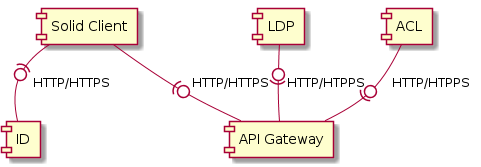
\includegraphics[width=1 \textwidth]{figures/component_diagram_2.png}
    \caption{Diagrama de Componentes Arquitetura 1}
    \end{center}
\end{figure}
\pagebreak

\subsection{Arquitetura 2}

\subsubsection{Explicação}

Esta arquitetura mantêm o conceito de API Gateway, mas introduz a adoção do protocolo SMQP como possível forma de actualização assíncrona das permissões de acesso a recursos no LDP.

Na prática o que isto permite é que a leitura das permissões seja independente da escrita das mesmas. E, desta forma, aplica-se o padrão CQRS (Command Query Responsability Segregation), contribuindo para um menor acoplamento entre o LDP e o ACL. Este conceito introduz indiretamente um outro: \emph{Eventual Consistency}, este por sua vez consiste na assunção de que alterações a um determinado modelo eventualmente induzirão num estado consistente no sistema como um todo. De acordo com o teorema de CAP, consistência é o parâmetro que devemos abdicar para conseguirmos escalabilidade e tolerância a falhas.

A utilização da arquitetura permite também a adoção do padrão \emph{Event Sourcing}, este consiste na persistência dos eventos de alteração de estado e permite que o estado do sistema seja obtido a qualquer momento pela "soma" das alterações de estado a que o mesmo foi sujeito.

\begin{figure}[h]
    \begin{center}
    % Requires \usepackage{graphicx}
    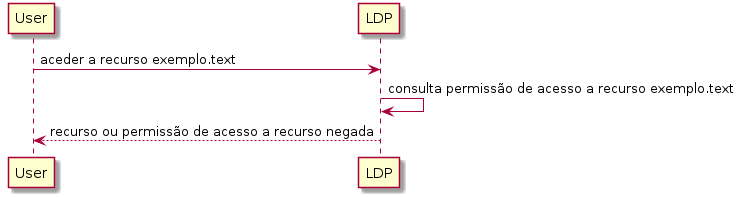
\includegraphics[width=1 \textwidth]{figures/arquitetura_2_access_resource}
    \caption{Diagrama de Sequência Arquitetura 2 - alterar permissão a recurso}
    \end{center}
\end{figure}

\begin{figure}[h]
    \begin{center}
    % Requires \usepackage{graphicx}
    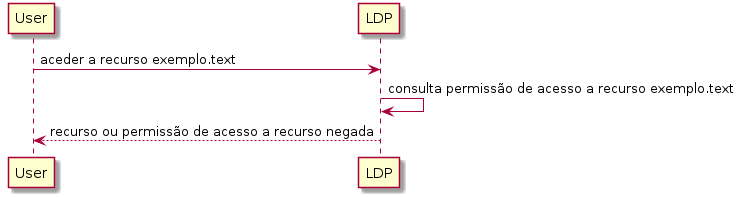
\includegraphics[width=1 \textwidth]{figures/arquitetura_2_access_resource}
    \caption{Diagrama de Sequência Arquitetura 2 - aceder recurso}
    \end{center}
\end{figure}


\subsubsection{Diagrama de componentes}
\begin{figure}[h]
    \begin{center}
    % Requires \usepackage{graphicx}
    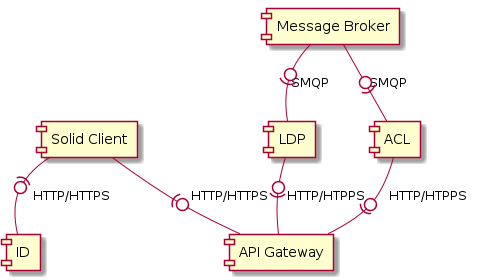
\includegraphics[width=1 \textwidth]{figures/component_diagram.png}
    \caption{Diagrama de Componentes Arquitetura 2}
    \end{center}
\end{figure}

\subsection{Comparação}

Ambas as arquiteturas 1 e 2 compreendem uma migração para micro-serviços, sustentada numa separação em serviços baseada em capacidades de negócio.
A grande diferença entre as duas é a introdução da componente Message Broker, este factor adiciona complexidade, mas por outro lado, garante um maior desacoplamento entre a componente LDP e a componente ACL, e garante também uma diminuição da latência na obtenção de um recurso.





